%	-------------------------------------------------------------------------------
% 
%
%
%
%
%
%
%
%
%
%	-------------------------------------------------------------------------------
	\documentclass[12pt, a4paper, oneside]{book}
%	\documentclass[12pt, a4paper, landscape, oneside]{book}

		% --------------------------------- 페이지 스타일 지정
		\usepackage{geometry}
%		\geometry{landscape=true	}
		\geometry{top 		=10em}
		\geometry{bottom		=10em}
		\geometry{left		=8em}
		\geometry{right		=8em}
		\geometry{headheight	=4em} % 머리말 설치 높이
		\geometry{headsep		=2em} % 머리말의 본문과의 띠우기 크기
		\geometry{footskip		=4em} % 꼬리말의 본문과의 띠우기 크기
% 		\geometry{showframe}
	
%		paperwidth 	= left + width + right (1)
%		paperheight 	= top + height + bottom (2)
%		width 		= textwidth (+ marginparsep + marginparwidth) (3)
%		height 		= textheight (+ headheight + headsep + footskip) (4)



		%	===================================================================
		%	package
		%	===================================================================
%			\usepackage[hangul]{kotex}				% 한글 사용
			\usepackage{kotex}						% 한글 사용
			\usepackage[unicode]{hyperref}			% 한글 하이퍼링크 사용
			\usepackage{amssymb,amsfonts,amsmath}	% 수학 수식 사용

			\usepackage{scrextend}					% 
		
		% ------------------------------ 개조식 문서 작성
			\usepackage{enumerate}			%
			\usepackage{enumitem}			%
			\usepackage{tabto}				%     tabto package
			\usepackage{tablists}			%	수학문제의 보기 등을 표현하는데 사용
										%	tabenum


		% ------------------------------ table 
			\usepackage{longtable}			%
			\usepackage{tabularx}			%

			\usepackage{setspace}			%
			\usepackage{booktabs}			% table
			\usepackage{color}				%
			\usepackage{multirow}			%
			\usepackage{boxedminipage}		% 미니 페이지
			\usepackage[pdftex]{graphicx}	% 그림 사용
			\usepackage[final]{pdfpages}	% pdf 사용
			\usepackage{framed}			% pdf 사용
			
			\usepackage{fix-cm}	
			\usepackage[english]{babel}
	
			\usepackage{tikz}%
			\usetikzlibrary{arrows,positioning,shapes}
			%\usetikzlibrary{positioning}
			



		% --------------------------------- 	page
			\usepackage{afterpage}			% 다음페이지가 나온면 어떻게 하라는 명령 정의 패키지
%			\usepackage{fullpage}			% 잘못 사용하면 다 흐트러짐 주의해서 사용
%			\usepackage{pdflscape}			% 
			\usepackage{lscape}			%	 


			\usepackage{blindtext}
	
		% --------------------------------- font 사용
			\usepackage{pifont}				%
			\usepackage{textcomp}
			\usepackage{gensymb}
			\usepackage{marvosym}






		% --------------------------------- 페이지 스타일 지정

		\usepackage[Sonny]		{fncychap}

			\makeatletter
			\ChNameVar	{\Large\bf}
			\ChNumVar		{\Huge\bf}
			\ChTitleVar	{\Large\bf}
			\ChRuleWidth	{0.5pt}
			\makeatother

%		\usepackage[Lenny]		{fncychap}
%		\usepackage[Glenn]		{fncychap}
%		\usepackage[Conny]		{fncychap}
%		\usepackage[Rejne]		{fncychap}
%		\usepackage[Bjarne]	{fncychap}
%		\usepackage[Bjornstrup]{fncychap}

		\usepackage{fancyhdr}
		\pagestyle{fancy}
		\fancyhead{} % clear all fields
		\fancyhead[LO]{\footnotesize \leftmark}
		\fancyhead[RE]{\footnotesize \leftmark}
		\fancyfoot{} % clear all fields
		\fancyfoot[LE,RO]{\large \thepage}
		%\fancyfoot[CO,CE]{\empty}
		\renewcommand{\headrulewidth}{1.0pt}
		\renewcommand{\footrulewidth}{0.4pt}
	
	
	
		% --------------------------------- 	section 스타일 지정
	
		\usepackage{titlesec}
		
		\titleformat*{\section}			{\large\bfseries}
		\titleformat*{\subsection}			{\normalsize\bfseries}
		\titleformat*{\subsubsection}		{\normalsize\bfseries}
		\titleformat*{\paragraph}			{\normalsize\bfseries}
		\titleformat*{\subparagraph}		{\normalsize\bfseries}
	
		\renewcommand{\thesection}			{\arabic{section}.}
		\renewcommand{\thesubsection}		{\thesection\arabic{subsection}.}
		\renewcommand{\thesubsubsection}	{\thesubsection\arabic{subsubsection}}
		
		\titlespacing*{\section} 			{0pt}{1.0em}{1.0em}
		\titlespacing*{\subsection}	  		{0ex}{1.0em}{1.0em}
		\titlespacing*{\subsubsection}		{0ex}{1.0em}{1.0em}
		\titlespacing*{\paragraph}			{0ex}{1.0em}{1.0em}
		\titlespacing*{\subparagraph}		{0ex}{1.0em}{1.0em}
	
	%	\titlespacing*{\section} 			{0pt}{0.0\baselineskip}{0.0\baselineskip}
	%	\titlespacing*{\subsection}	  		{0ex}{0.0\baselineskip}{0.0\baselineskip}
	%	\titlespacing*{\subsubsection}		{6ex}{0.0\baselineskip}{0.0\baselineskip}
	%	\titlespacing*{\paragraph}			{6pt}{0.0\baselineskip}{0.0\baselineskip}
	

		% --------------------------------- recommend		섹션별 페이지 상단 여백
		\newcommand{\SectionMargin}			{\newpage  \null \vskip 2cm}
		\newcommand{\SubSectionMargin}		{\newpage  \null \vskip 2cm}
		\newcommand{\SubSubSectionMargin}	{\newpage  \null \vskip 2cm}


	
		% --------------------------------- 장의 목차
		\usepackage{minitoc}
		\setcounter{minitocdepth}{1}    	% Show until subsubsections in minitoc
		\setlength{\mtcindent}{12pt} 		% default 24pt
	
	
		% --------------------------------- 	문서 기본 사항 설정
		\setcounter{secnumdepth}{3} 		% 문단 번호 깊이
		\setcounter{tocdepth}{3} 			% 문단 번호 깊이
		\setlength{\parindent}{0cm} 		% 문서 들여 쓰기를 하지 않는다.
		

		% --------------------------------- 	찾아보기
		\usepackage{makeidx}
		\makeindex

		% --------------------------------- 	줄간격 설정
		\doublespace
%		\onehalfspace
%		\singlespace
		
		
% 	============================================================================== List global setting
%		\setlist{itemsep=1.0em}
	
% 	============================================================================== enumi setting

%		\renewcommand{\labelenumi}{\arabic{enumi}.} 
%		\renewcommand{\labelenumii}{\arabic{enumi}.\arabic{enumii}}
%		\renewcommand{\labelenumii}{(\arabic{enumii})}
%		\renewcommand{\labelenumiii}{\arabic{enumiii})}


	%	-------------------------------------------------------------------------------
	%		Vertical and Horizontal spacing
	%	-------------------------------------------------------------------------------
		\setlist[enumerate,1]	{ leftmargin=8.0em, rightmargin=0.0em, labelwidth=0.0em, labelsep=0.0em }
		\setlist[enumerate,2]	{ leftmargin=8.0em, rightmargin=0.0em, labelwidth=0.0em, labelsep=0.0em }
		\setlist[enumerate,3]	{ leftmargin=8.0em, rightmargin=0.0em, labelwidth=0.0em, labelsep=0.0em }
		\setlist[enumerate]	{ 	itemsep=0.0em, 
								leftmargin=6.0ex, 
								rightmargin=0.0em, 
								labelwidth=0.0em, 
								labelsep=4.0ex 
							}


	%	-------------------------------------------------------------------------------
	%		Label
	%	-------------------------------------------------------------------------------
%		\setlist[enumerate,1]{ label=\arabic*., ref=\arabic* }
%		\setlist[enumerate,1]{ label=\emph{\arabic*.}, ref=\emph{\arabic*} }
%		\setlist[enumerate,1]{ label=\textbf{\arabic*.}, ref=\textbf{\arabic*} }   	% 1.
%		\setlist[enumerate,1]{ label=\textbf{\arabic*)}, ref=\textbf{\arabic*)} }		% 1)
		\setlist[enumerate,1]{ label=\textbf{(\arabic*)}, ref=\textbf{(\arabic*)} }	% (1)
		\setlist[enumerate,2]{ label=\textbf{\arabic*)}, ref=\textbf{\arabic*)} }		% 1)
		\setlist[enumerate,3]{ label=\textbf{\arabic*.}, ref=\textbf{\arabic*.} }		% 1.

%		\setlist[enumerate,2]{ label=\emph{\alph*}),ref=\theenumi.\emph{\alph*} }
%		\setlist[enumerate,3]{ label=\roman*), ref=\theenumii.\roman* }


% 	============================================================================== itemi setting


	%	-------------------------------------------------------------------------------
	%		Vertical and Horizontal spacing
	%	-------------------------------------------------------------------------------
		\setlist[itemize]{itemsep=0.0em}


	%	-------------------------------------------------------------------------------
	%		Label
	%	-------------------------------------------------------------------------------
		\renewcommand{\labelitemi}{$\bullet$}
		\renewcommand{\labelitemii}{$\cdot$}
		\renewcommand{\labelitemiii}{$\diamond$}
		\renewcommand{\labelitemiv}{$\ast$}		




		% --------------------------------- recommend  글자 색깔지정 명령
		\newcommand{\red}		{\color{red}}			% 글자 색깔 지정
		\newcommand{\blue}		{\color{blue}}		% 글자 색깔 지정
		\newcommand{\black}	{\color{black}}		% 글자 색깔 지정
		\newcommand{\superscript}[1]{${}^{#1}$}

	
	
		% --------------------------------- 환경 정의 : 박스 치고 안의 글자 빨간색

			\newenvironment{BoxRedText}
			{ 	\setlength{\fboxsep}{12pt}
				\begin{boxedminipage}[c]{1.0\linewidth}
				\color{red}
			}
			{ 	\end{boxedminipage} 
				\color{black}
			}
			
%		\setmainhangulfont[BoldFont=HY견고딕]{한컴돋움}
%		\setsanshangulfont{HY견고딕}
%		\setmonohangulfont{한컴돋움}
			
			

% ------------------------------------------------------------------------------
% Begin document (Content goes below)
% ------------------------------------------------------------------------------
	\begin{document}
	
			\dominitoc
			

			\title{typing}
			\author{김대희}
			\date{2015년 8월}
			\maketitle


			\tableofcontents
			\listoffigures
			\listoftables

			



% ===========================================================	part		=============
		\addtocontents{toc}{\protect\newpage}
		\part{일반 사항}

% ================================================= chapter 	====================
	\newpage
	\chapter{chapter name}


	% -------------------------------------- page -------------------
	%	\nomtcrule         		% removes rules = horizontal lines
	%	\nomtcpagenumbers  % remove page numbers from minitocs
		\newpage
		\minitoc				% Creating an actual minitoc
	%	\doublespace


	% ------------------------------------------ section ------------ 
	\newpage  \null
	\section{section name}






	% ------------------------------------------ section ------------ 
	\SectionMargin
	\section{상호참조}


		\begin{verbatim}
			\label{참조기호}	% 참조대상이 되는 부정
			\ref{참조할 기호}	% 참조대상이 되는 번호
			\pageref{참조기호}	% 참조대상이 되는 쪽번호
		\end{verbatim}



	% ------------------------------------------ section ------------ 
	\SectionMargin
	\section{하이퍼링크 삽입}

		\setlength{\fboxrule}{2pt} 
		\setlength{\fboxsep} {1em} 
		\begin{boxedminipage}[c,fboxrule=10pt,fboxsep=12pt]{1.0\linewidth}
		\begin{verbatim}
		\url{하이퍼링크}
		\end{verbatim}
		\end{boxedminipage} \\



	\begin{enumerate}[itemsep=0.0pt]
	\item	\url{http://www.band.us/#/band/53125310} 
	\item	\url{http://www.seoyeong.co.kr/}
	\item	\url{http://symsone.seoyeong.co.kr}
	\item	\url{http://syerp.seoyeong.co.kr/}

	\end{enumerate}


	% ------------------------------------------ section ------------ 
	\SectionMargin
	\section{이메일 주소 입력}



		email \href{mailto:me@somewhere.com}{me@somewhere.com} \\
		email \href{mailto:someone@somewhere.com}{someone@somewhere.com} 





% 	================================================= chapter 	====================
%
%	-------------------------------------------------------------------------------
%	\newpage
%	\chapter{사용 예제 테스트}
%
%		\Blinddocument
%				



% 	================================================= chapter 	==================== geometry
%		geometry test
%	-------------------------------------------------------------------------------
	\newpage
	\chapter{geometry test}

		\newpage
		\section{geometry test}

		\clearpage
		\newgeometry{left=3cm, right=1cm, bottom=1.2cm, showframe}
		newgeometry\{left=3cm, right=1cm, bottom=1.2cm,showframe\}

		\clearpage
		\restoregeometry
		restoregeometry



		\clearpage
		\newgeometry{landscape=TRUE, left=6cm, right=6cm, bottom=1.2cm,showframe=true}

		newgeometry\{landscape=true, left=6cm, right=6cm, bottom=1.2cm,showframe\}

		\clearpage
		\newgeometry{landscape=TRUE, paper=a5paper}
		landscape=TRUE, paper=a5paper, margin=10pt


		\clearpage
		\newgeometry{landscape=true, paper=a5paper}
		landscape=TRUE, paper=a5paper, margin=10pt

		\clearpage
		\restoregeometry
		restoregeometry


	%	----------------------------------------------------------- 
		\clearpage

		\begin{landscape}
		pdflscape package   landscape
		\end{landscape}
		restoregeometry

















% ===========================================================	part		=============
		\addtocontents{toc}{\protect\newpage}
		\part{part1}



				
% 	================================================= chapter 	====================
%
%	-------------------------------------------------------------------------------
	\newpage
	\chapter{폰트 테스트}

		\newpage
		\section{폰트 테스트}

			\begin{itemize}
			\item \textrm{\large serif(main)은 `서울한강L(한글)'과 `Constantia'(영문)}
			\item \textrm{\large serif의 漢字는 `함초롬 바탕 LVT'}
			\item \textsf{\large sans serif는 `a고래야놀자(한글)'과 `Chinacat'(영문)}
			\item \texttt{\large typewriter는 `a하늘산책M(한글)'과 `The Great Escape'(영문)}
			\end{itemize}







	% ==============================================================================	
	%	Alignement 
	% ==============================================================================	
	\SectionMargin
	\section{Alignement : 명령 지정 후 부터 문서 전체에 대해서 }



	\begin{verbatim}
		\raggedright	% 오른쪽 정렬
		\raggedleft	% 왼쪽 정렬
		\centering	% 가운데 정렬
	\end{verbatim}



	\SectionMargin
	\section{Alignement : 지정 범위내에서만}

	%	----------------------------------------------------------
		\subsection{flushright}

			\begin{verbatim}
				\begin{flushright}
				\end{flushright}
			\end{verbatim}
		
				\begin{flushright}
				오른쪽 정렬
				\end{flushright}

	%	----------------------------------------------------------
		\subsection{flushleft}

			\begin{verbatim}
				\begin{flushleft}
				\end{flushleft}
			\end{verbatim}
		
				\begin{flushleft}
				왼쪽 정렬
				\end{flushleft}
		
	%	----------------------------------------------------------
		\subsection{center}
		
			\begin{verbatim}
				\begin{center}
				\end{center}
			\end{verbatim}
		
				\begin{center}
				가운데 정렬
				\end{center}




	% ==============================================================================	
	%	Alignement 
	% ==============================================================================	
	\SectionMargin
	\section{Alignement }


	%	----------------------------------------------------------
		\subsection{hspace}

			\begin{verbatim}
				\hspace{40mm}
			\end{verbatim}
		
				\hspace{40mm} ============

	%	----------------------------------------------------------
		\subsection{hfill}

		==========
		\hfill 
		==========
		==========


		
	%	----------------------------------------------------------
		\subsection{vspace}

			\begin{verbatim}
				\vspace{10mm}
			\end{verbatim}

			====================================\\
			\vspace{10mm}
			====================================\\
			\vspace{10mm}
			====================================\\
			====================================\\
			====================================\\
			====================================\\
			====================================\\

	%	----------------------------------------------------------
		\newpage
		\subsection{vill}

		==========
		\vfill 
		==========
		==========


% ===========================================================	part		=============
		\addtocontents{toc}{\protect\newpage}
		\part{List}


% 	================================================= chapter 	====================
%
%	-------------------------------------------------------------------------------
	\newpage
	\chapter{List}
	\newpage  \null

	% ==============================================================================	
	%	itemize
	% ==============================================================================	

	\newpage
	\section{itemize}

		% ----------------------------- itemize
			\begin{itemize}
			\item	
			\item	
			\item	
			\item	
			\item	
			\item	
			\end{itemize}
			
			\begin{itemize}[topsep=0.0em,itemsep=0.0em]
			\item	
			\end{itemize}	


			[itemsep=-0.5em]
			[topsep=-1.0em,			]


			\begin{itemize}[	topsep=0.0em,itemsep=0.0em,
							leftmargin=4em, labelsep=3em ]
			\item	
			\end{itemize}	

			
		% ----------------------------- itemize
		\def\TStart{	\setlength{\fboxsep}{12pt}
					\begin{boxedminipage}[c]{1.0\linewidth}
					\begin{itemize}[topsep=0.0em,itemsep=0.0em]
					}
		\def\TEnd{	\end{itemize}	
					\end{boxedminipage}\\
					}
		\TStart
		\item 1 
		\item 2 
		\TEnd

		\setlength{\fboxsep}{12pt}
		\begin{boxedminipage}[c]{1.0\linewidth}
		\end{boxedminipage}\\

	% ==============================================================================	
	%	enumerate
	% ==============================================================================	

	\newpage
	\section{enumerate}

		% ----------------------------- enumerate
		\begin{enumerate}
		\setlength\itemsep{-1.0em}
		\item	enumerate test 1
		\item	enumerate test 2
		\item	enumerate test 3
		\item	enumerate test 4
			\begin{enumerate}
			\setlength\itemsep{-1.0em}
			\item	enumerate test 1
			\item	enumerate test 2
			\item	enumerate test 3
			\item	enumerate test 4
				\begin{enumerate}
				\setlength\itemsep{-1.0em}
				\item	enumerate test 1
				\item	enumerate test 2
				\item	enumerate test 3
				\item	enumerate test 4
				\item	enumerate test 5
				\item	enumerate test 6
				\end{enumerate}
			\item	enumerate test 5
			\item	enumerate test 6
			\end{enumerate}
		\item	enumerate test 5
		\item	enumerate test 6
		\end{enumerate}
		


	\newpage

		\subsection{enumerate : label}
		% -------------------------------------
		% 	arabic*
		% -------------------------------------
		\begin{enumerate}[ label=\arabic*)]
		\setlength\topsep{0.0em}
		\setlength\itemsep{-1.0em}
		\item	enumerate test 1
		\item	enumerate test 2
		\item	enumerate test 3
		\end{enumerate}

		% ----------------------------- enumerate
		\begin{enumerate}[ label=\arabic*)]
		\item	enumerate test 1
		\item	enumerate test 2
		\item	enumerate test 3
		\item	enumerate test 4
		\item	enumerate test 5
		\item	enumerate test 6
		\end{enumerate}


	\newpage

		% ----------------------------- enumerate
		\begin{enumerate}
		\setlength\topsep{0.0em}
		\setlength\itemsep{-1.0em}
		\setlength\labelwidth{0.0cm}
		\setlength\labelsep{1cm}

		\item	enumerate test 1
		\item	enumerate test 2
		\item	enumerate test 3
		\item	enumerate test 4
		\item	enumerate test 5
		\item	enumerate test 6
		\end{enumerate}
		

		% ----------------------------- enumerate
		\begin{enumerate}[ leftmargin=2cm ]
		\setlength\topsep{0.0em}
		\setlength\itemsep{-1.0em}
		\setlength\labelwidth{0.0cm}
		\setlength\labelsep{1cm}

		\item	enumerate test 1
		\item	enumerate test 2
		\item	enumerate test 3
		\item	enumerate test 4
		\item	enumerate test 5
		\item	enumerate test 6
		\end{enumerate}



		\subsection{enumerate : defalult}
		% ----------------------------- enumerate
		\begin{enumerate}[leftmargin=4cm]
		\setlength\topsep{0.0em}
		\setlength\itemsep{0.0em}
		\setlength\leftmargin{0cm}
		\setlength\rightmargin{6cm}

		\setlength\labelsep  {1.0cm}
		\setlength\labelwidth{0.0cm}
		\setlength\listparindent{0.0em}

		\item	enumerate test 1
		\item	enumerate test 2
		\item	enumerate test 3
		\item	enumerate test 4
		\item	enumerate test 5
		\item	enumerate test 6
		\end{enumerate}


	\newpage

		% ----------------------------- enumerate
		\begin{enumerate}
		\setlength\leftmargin{8cm}
		\setlength\rightmargin{10cm}
		\item	보강토체를 따른 활동(성토체내의 흙과 흙 사이의 내부마찰각) 
		\item	기초지반을 따른 활동(성토체흙과 기초지반흙과의 마찰각) 
		\item	최하단 토목섬유 보강재와 흙 사이의 경계면을 따른 활동 
		\end{enumerate}

		% ----------------------------- enumerate
		\begin{enumerate}[leftmargin=4cm, rightmargin=4cm]
		\item	보강토체를 따른 활동(성토체내의 흙과 흙 사이의 내부마찰각) 
		\item	기초지반을 따른 활동(성토체흙과 기초지반흙과의 마찰각) 
		\item	최하단 토목섬유 보강재와 흙 사이의 경계면을 따른 활동 
		\end{enumerate}

	\newpage

		% ----------------------------- enumerate
		\begin{dingautolist}{172}
		\setlength\leftmargin{8cm}
		\setlength\rightmargin{10cm}
		\item	보강토체를 따른 활동(성토체내의 흙과 흙 사이의 내부마찰각) 
		\item	기초지반을 따른 활동(성토체흙과 기초지반흙과의 마찰각) 
		\item	최하단 토목섬유 보강재와 흙 사이의 경계면을 따른 활동 
		\end{dingautolist}

		% ----------------------------- enumerate
		\begin{dingautolist}{172}
		\item	보강토체를 따른 활동(성토체내의 흙과 흙 사이의 내부마찰각) 
		\item	기초지반을 따른 활동(성토체흙과 기초지반흙과의 마찰각) 
		\item	최하단 토목섬유 보강재와 흙 사이의 경계면을 따른 활동 
		\end{dingautolist}

		% ----------------------------- 사용자 정의
		\begin{enumerate}[label=\bfseries Exercise \arabic*:]
		\setlength\itemsep{1em}
		 \item 5 + 7 = 12
		 \item 9 + 1 = 10
		 \item 2 $\times$ 2 = 4
		\end{enumerate}

	% ==============================================================================	
	%	description
	% ==============================================================================	
	%
	%	left margin은 style=sameline에서만 적용된다.
	%

	\newpage
	\section{description}


			%	labelindent=0pt: to have a flush left margin;



		\subsection{description : defalult}
			% ----------------------------- description
			\paragraph{ align = left }
			\begin{description}[topsep=0.0em, itemsep=-1.0em, leftmargin=14cm,align=left]
			\item	[description 1]	description test 1
			\item	[description]		description test 2
			\item	[descrip]			description test 3
			\item	[descrip]			description test 4
			\item	[desc]			description test 5
			\item	[d]				description test 6
			\end{description}



			\paragraph{ align = right }
			\begin{description}[topsep=0.0em, itemsep=-1.0em, leftmargin=14cm,align=right]
			\item	[description 1]	description test 1
			\item	[description]		description test 2
			\item	[descrip]			description test 3
			\item	[descrip]			description test 4
			\item	[desc]			description test 5
			\item	[d]				description test 6
			\end{description}

		\newpage
		\subsection{description : style=standard}
			% ----------------------------- description
			\paragraph{ align = left }
			\begin{description}[style=standard, align=left]
			\setlength\topsep{0.0em}
			\setlength\itemsep{-1.0em}
			\setlength\labelsep{1cm}
			\item	[description 1]	description test 1
			\item	[description]		description test 2
			\item	[descrip]			description test 3
			\item	[descrip]			description test 4
			\item	[desc]			description test 5
			\item	[d]				description test 6
			\end{description}



			\paragraph{ align = right }
			\begin{description}[style=standard, align=right]
			\setlength\topsep{0.0em}
			\setlength\itemsep{-1.0em}
			\setlength\leftmargin{4cm}
			\setlength\labelsep{1cm}
			\item	[description 1]	description test 1
			\item	[description]		description test 2
			\item	[descrip]			description test 3
			\item	[descrip]			description test 4
			\item	[desc]			description test 5
			\item	[d]				description test 6
			\end{description}

			\paragraph{ align = parleft }
			\begin{description}[style=standard, align=parleft]
			\setlength\topsep{0.0em}
			\setlength\itemsep{-1.0em}
			\setlength\leftmargin{4cm}
			\setlength\labelsep{1cm}

			\item	[description 1]	description test 1
			\item	[description]		description test 2
			\item	[descrip]			description test 3
			\item	[descrip]			description test 4
			\item	[desc]			description test 5
			\item	[d]				description test 6
			\end{description}



			\paragraph{ align = parleft }
			\begin{description}[style=standard, align=parleft, leftmargin=6cm]
			\setlength\topsep{0.0em}
			\setlength\labelsep{1cm}
			\setlength\itemsep{-1.0em}
			\setlength\labelwidth{1.2cm}

			\item	[description 1]	description test 1
			\item	[description]		description test 2
			\item	[descrip]			description test 3
			\item	[descrip]			description test 4
			\item	[desc]			description test 5
			\item	[d]				description test 6
			\end{description}


		\subsection{description : unboxed}
			% ----------------------------- description
			\begin{description}[style=unboxed]
			\setlength\topsep{0.0em}
			\setlength\itemsep{-1.0em}
			\setlength\leftmargin{12cm}
			\setlength\labelwidth{2cm}
			\setlength\labelsep{2em}


			\item	[description 1]	description test 1
			\item	[description]		description test 2
			\item	[descrip]			description test 3
			\item	[descrip]			description test 4
			\item	[desc]			description test 5
			\item	[d]				description test 6
			\end{description}


		\newpage
		\subsection{description : nextline}
			% ----------------------------- description
			\begin{description}[style=nextline, align=left]
			\setlength\topsep{0.0em}
			\setlength\itemsep{-1.0em}

			\item	[description 1]	description test 1
			\item	[description]		description test 2
			\item	[descrip]			description test 3
			\item	[descrip]			description test 4
			\item	[desc]			description test 5
			\item	[d]				description test 6
			\end{description}


			% ----------------------------- description
			\begin{description}[style=nextline]
			\setlength\topsep{0.0em}
			\setlength\itemsep{-1.0em}

			\item	[description 1]	description test 1
			\item	[description]		description test 2
			\item	[descrip]			description test 3
			\item	[descrip]			description test 4
			\item	[desc]			description test 5
			\item	[d]				description test 6
			\end{description}




			% ----------------------------- description
			%	sameline
			% ----------------------------- description

		\newpage
		\subsection{description : sameline}
			% ----------------------------- description
			\begin{description}[style=sameline]
			\setlength\topsep{0.0em}
			\setlength\itemsep{-1.0em}
			\item	[description 1]	description test 1
			\item	[description]		description test 2
			\item	[descrip]			description test 3
			\item	[descrip]			description test 4
			\item	[desc]			description test 5
			\item	[d]				description test 6
			\end{description}


			\begin{description}[style=sameline, leftmargin=2cm]
			\setlength\topsep{0.0em}
			\setlength\itemsep{-0.5em}
%\singlespacing
%\onehalfspacing
%\doublespacing

			\item	[description 1]	description test 1
			\item	[description]		description test 2
			\item	[descrip]			description test 3
			\item	[descrip]			description test 4
			\item	[desc]			description test 5
			\item	[d]				description test 6
			\item[$b$] Taxa agregada de bits alcançável para o sistema
			\item[$H(f)$] Espectro do canal
			\item[$H_k$] Ganho do $k$-ésimo subcanal
			\item[$P_x$] Potência total de transmissão
			\item[$s_k$] Densidade espectral de potência do sinal no $k$-ésimo subcanal
			\item[$Sx(f)$] Densidade espectral de potência do sinal na frequência contínua
			\item[$Sn(f)$] Densidade espectral de potência do AWGN na frequência contínua
			\item[1]	보강토체를 따른 활동(성토체내의 흙과 흙 사이의 내부마찰각) 
					보강토체를 따른 활동(성토체내의 흙과 흙 사이의 내부마찰각) 
			\item[2]	기초지반을 따른 활동(성토체흙과 기초지반흙과의 마찰각) 
			\item[3]	최하단 토목섬유 보강재와 흙 사이의 경계면을 따른 활동 

			\end{description}

		\newpage
		
		\subsection{description : align=left}
		% ----------------------------- description
		\begin{description}[labelsep=3em, align=left]
		\setlength\topsep{0.0em}
		\setlength\itemsep{-1.0em}

		\item[$b$] Taxa agregada de bits alcançável para o sistema
		\item[$H(f)$] Espectro do canal
		\item[$H_k$] Ganho do $k$-ésimo subcanal
		\item[$P_x$] Potência total de transmissão
		\item[$s_k$] Densidade espectral de potência do sinal no $k$-ésimo subcanal
		\item[$Sx(f)$] Densidade espectral de potência do sinal na frequência contínua
		\item[$Sn(f)$] Densidade espectral de potência do AWGN na frequência contínua
		\end{description}

		\subsection{description : align=right}
		% ----------------------------- description
		\begin{description}[labelsep=3em, align=right]
		\setlength\topsep{0.0em}
		\setlength\itemsep{-1.0em}

		\item[$b$] Taxa agregada de bits alcançável para o sistema
		\item[$Sn(f)$] Densidade espectral de potência do AWGN na frequência contínua
		\item[$\text{SNR}_k$] Razão sinal-ruído no subcanal $k$
		\item[$\mathbf{X}$] Vetor correspondente ao símbolo DMT
		\item[$\mathbf{X}_+$] Vetor de subsímbolos dos tons positivos do símbolo DMT.
		\item[$X_k$] Subsímbolo no $k$-ésimo tom do símbolo DMT
		\item[$\Gamma$] \textsl[Gap] de SNR a capacidade
		\item[$\Delta f$] Largura de banda do subcanal (espaçamento tonal).
		\item[$\sigma_k$] Densidade espectral de potência do AWGN no $k$-ésimo subcanal
		\end{description}



	% ==============================================================================	
	%	paralist
	% ==============================================================================	
	%

	\newpage
	\section{paralist}





	% ==============================================================================	
	%	TAB
	% ==============================================================================	
	%

	\newpage
	\section{tabbing}


		\begin{boxedminipage}[c,fboxrule=10pt,fboxsep=12pt]{1.0\linewidth}
		\begin{itemize}
		\item[]	\textbackslash begin \{tabbing\}
		\item[]	text \textbackslash = more text \textbackslash = still more text \textbackslash = last text \textbackslash\textbackslash 
		\item[]	\textbackslash end \{tabbing\}
		\end{itemize}
		\end{boxedminipage} \\


		\paragraph{set the tab position}


		\begin{tabbing}
		\hspace{2cm}	\= \hspace{2cm}	\= \hspace{2cm}	\\
		second row 	\> text-- 	\> more \\
		second row 	\> text-- 	\> more \\
		\end{tabbing}

		\begin{tabbing}
		\hspace{2cm}	\=\hspace{2cm}	\=\hspace{2cm}\\
		second row 	\>  		\> more \\
		second row 	\>  		\> more \\
		\end{tabbing}

		\paragraph{Tabbing commands}
		\begin{description}[itemsep=-0.5em,style=sameline]
		\item [\textbackslash =] set tab
		\item [\textbackslash $>$] advance to next tab stop
		\item [\textbackslash $<$]
		\item [\textbackslash $+$] indent; move margin right
		\item [\textbackslash $-$] unindent; move margin left
		\item [\textbackslash ']
		\item [\textbackslash `]
		\item [\textbackslash \textbackslash] end of line; newline
		\item [\textbackslash kill] ignore preceding text; use only for spacing
		\end{description}




	% ==============================================================================	
	%	tabto
	% ==============================================================================	
	%

	\newpage
	\section{tabto package}


		\NumTabs{5}
		set tab \tab
		set tab \tab
		set tab \tab
		set tab \tab
		set tab \tab
		set tab \tab
		set tab \tab
		set tab \tab

		\NumTabs{3}
		set tab \tab
		set tab \tab
		set tab \tab
		set tab \tab
		set tab \tab
		set tab \tab
		set tab \tab
		set tab \tab


	% ==============================================================================	
	%	TAB enum : 문제 풀이의 보기 항목
	% ==============================================================================	
	%	tablists package
	%

	\newpage
	\section{tabenum}



		\begin{tabenum}[\bfseries1)]%
		\tabenumitem 		$z=\displaystyle\frac xy$
		\tabenumitem 		$z=\displaystyle\frac xy$\\
		\tabenumitem 		$z=\displaystyle\frac xy$
		\tabenumitem 		$z=\displaystyle\frac xy$\\
		\tabenumitem 		$z=\displaystyle\frac xy$ 
		\skipitem
		\tabenumitem 		$6 z=\displaystyle\frac xy$\\	
		\item			$7 z=\displaystyle\frac xy$
		\noitem			$2^x=9$
		\item			$2^x=9 noitem$\cr
		\item			$2^x=9$\cr
		\item			$2^x=9$\cr
		\item			$2^x=9$\cr
		\tabenumitem		$3^{2x+3}=16 $
		\tabenumitem		$z=2x^2+4y^2$\par
		\tabenumitem		$u=\sqrt{x^2+y^2+z^2}$
		\tabenumitem		$v=gt+\displaystyle\frac{g}{4}t$;\\[1ex]
		\tabenumitem		$v=gt+\frac{g}{4}t$;\\[1ex]
%		\tabenumitem		$u=2ˆ{5x-3y+z}$;
%		\tabenumitem		$w=(v+7)ˆ2+(u-3)ˆ2$;
%		\tabenumitem		$5ˆx=\displaystyle\frac{4}{3} ;$
%		\tabenumitem		$z=(x+1)ˆ2+yˆ2$;\\*
%		\tabenumitem		$2+5+8+ \ldots +(3n+2)=155$, $n\in \mathrm{N};$
%		\tabenumitem		$t=5uˆ2+8vˆ2$;
		\end{tabenum}











% ===========================================================	part		=============
		\addtocontents{toc}{\protect\newpage}
		\part{Box}




% 	================================================= chapter 	====================
%		box
%	-------------------------------------------------------------------------------
	\newpage
	\chapter{box}

	% -------------------------------------- page -------------------
	%	\nomtcrule         		% removes rules = horizontal lines
	%	\nomtcpagenumbers  % remove page numbers from minitocs
		\newpage
		\minitoc				% Creating an actual minitoc
	%	\doublespace



	% ------------------------------------------------------------------------------
	%	par box
	% ------------------------------------------------------------------------------
	\SectionMargin
	\section{parbox}

		\setlength{\fboxrule}{2pt} 
		\setlength{\fboxsep} {1em} 

		\begin{boxedminipage}[c,fboxrule=10pt,fboxsep=12pt]{1.0\linewidth}
		\begin{verbatim}
		\parbox[position][height][inner-pos]{width}{text}
		\end{verbatim}
		\end{boxedminipage} \\

		\paragraph{position}
		\begin{itemize}[itemsep=0.0em]
		\item	t --- text is placed at the top of the box.
		\item	c --- text is centred in the box.
		\item	b --- text is placed at the bottom of the box.
		\item	s --- stretch vertically. The text must contain vertically stretchable space for this to work.
		\end{itemize}


		\setlength{\fboxrule}{2pt} 
		\setlength{\fboxsep} {1em} 

		\subsection{ center }
		\begin{parbox}[c]{0.7\linewidth}
{mini page	 mini page	 mini page	 mini page	 mini page	 mini page	 mini page	 mini page	 mini page	 mini page	 mini page	 mini page	 mini page	 mini page	 mini page	 mini page	 mini page	 mini page	 mini page	 mini page	 mini page	 mini page	 mini page	 mini page	 mini page	 mini page	 mini page	 mini page	 mini page	 mini page	 mini page	 mini page	 mini page	 mini page}
		\end{parbox} 


		\newpage
		\subsection{ parbox와 paragraph를 혼합한 응용}
		\paragraph{ bottom의 응용 }
		\begin{parbox}[b]{0.8\linewidth}
{mini page	 mini page	 mini page	 mini page	 mini page	 mini page	 mini page	 mini page	 mini page	 mini page	 mini page	 mini page	 mini page	 mini page	 mini page	 mini page	 mini page	 mini page	 mini page	 mini page	 mini page	 mini page	 mini page	 mini page	 mini page	 mini page	 mini page	 mini page	 mini page	 mini page	 mini page	 mini page	 mini page	 mini page}
		\end{parbox} 

		\paragraph{ top의 응용 }
		\begin{parbox}[t]{0.8\linewidth}
{mini page	 mini page	 mini page	 mini page	 mini page	 mini page	 mini page	 mini page	 mini page	 mini page	 mini page	 mini page	 mini page	 mini page	 mini page	 mini page	 mini page	 mini page	 mini page	 mini page	 mini page	 mini page	 mini page	 mini page	 mini page	 mini page	 mini page	 mini page	 mini page	 mini page	 mini page	 mini page	 mini page	 mini page}
		\end{parbox} 



	% ------------------------------------------------------------------------------
	%	mbox
	% ------------------------------------------------------------------------------
	\SectionMargin
	\section{mbox}


		\begin{boxedminipage}[c,fboxrule=10pt,fboxsep=12pt]{1.0\linewidth}
		\begin{verbatim}
		\mbox{text}
		\end{verbatim}
		\end{boxedminipage} \\

		\mbox{mbox mbox mbox mbox mbox mbox mbox}


	% ------------------------------------------------------------------------------
	%	fbox
	% ------------------------------------------------------------------------------
	\SectionMargin
	\section{fbox}


		\begin{boxedminipage}[c,fboxrule=10pt,fboxsep=12pt]{1.0\linewidth}
		\begin{verbatim}
		\fbox{text}
		\end{verbatim}
		\end{boxedminipage} \\

		\fbox{mbox mbox mbox mbox mbox mbox mbox}


	% ------------------------------------------------------------------------------
	%	pbox
	% ------------------------------------------------------------------------------
	\SectionMargin
	\section{pbox}


		\begin{boxedminipage}[c,fboxrule=10pt,fboxsep=12pt]{1.0\linewidth}
		\begin{verbatim}
		\pbox[b]{\textwidth}{my text}
		\end{verbatim}
		\end{boxedminipage} \\

%		\pbox{mbox mbox mbox mbox mbox mbox mbox}
%		\pbox{\textwidth}{my text}
%		\pbox{\textwidth}{my text}
%		\pbox{\textwidth}{my text}



	% ------------------------------------------------------------------------------
	%	save box
	% ------------------------------------------------------------------------------
	\SectionMargin
	\section{save box}





	% ------------------------------------------------------------------------------
	%	rotate box
	% ------------------------------------------------------------------------------
	\SectionMargin
	\section{rotate box}

	% ------------------------------------------------------------------------------
	%	colorbox and fcolorbox
	% ------------------------------------------------------------------------------
	\SectionMargin
	\section{colorbox and fcolorbox}


	% ------------------------------------------------------------------------------
	%	resize box
	% ------------------------------------------------------------------------------
	\SectionMargin
	\section{resize box}

		\resizebox{1em}{2em}{Dunhill style} \\
		\resizebox{2em}{2em}{Dunhill style} \\
		\resizebox{3em}{2em}{Dunhill style} \\
		\resizebox{4em}{2em}{Dunhill style} \\
		\resizebox{5em}{2em}{Dunhill style} \\
		\resizebox{6em}{2em}{Dunhill style} \\
		\resizebox{7em}{2em}{Dunhill style} \\
		\resizebox{8em}{2em}{Dunhill style} \\

		\resizebox{8em}{1ex}{Dunhill style} \\
		\resizebox{8em}{2ex}{Dunhill style} \\
		\resizebox{8em}{3ex}{Dunhill style} \\
		\resizebox{8em}{4ex}{Dunhill style} \\
		\resizebox{8em}{5ex}{Dunhill style} \\
		\resizebox{8em}{6ex}{Dunhill style} \\


	% ------------------------------------------------------------------------------
	%	scale box
	% ------------------------------------------------------------------------------
	\SectionMargin
	\section{scale box}


		\scalebox{10}{Giant}\\
		\scalebox{1}{화이팅!}\\
		\scalebox{2}{화이팅!}\\
		\scalebox{3}{화이팅!}\\
		\scalebox{4}{화이팅!}\\
		\scalebox{5}{화이팅!}\\
		\scalebox{6}{화이팅!}\\



	% ------------------------------------------------------------------------------
	%	fancybox
	% ------------------------------------------------------------------------------
	\SectionMargin
	\section{fancy box}


	\subsection{double box}

	\subsection{oval box}

	\subsection{shadow box}





	% ------------------------------------------------------------------------------
	%	makebox
	% ------------------------------------------------------------------------------
	\SectionMargin
	\section{makebox}


		\begin{boxedminipage}[c,fboxrule=10pt,fboxsep=12pt]{1.0\linewidth}
		\begin{verbatim}
		\makebox [ width ] [ pos ] {text}
		\end{verbatim}
		\end{boxedminipage} \\

		\paragraph{position}
		\begin{itemize}[itemsep=0.0em]
		\item	c : center
		\item	l : flushleft
		\item	r : flushright
		\item	s : spread
		\end{itemize}

		\makebox[0.4\linewidth][s]
		{makebox makebox makebox makebox makebox makebox makebox makebox makebox makebox makebox makebox makebox makebox makebox }

		c : \makebox[0.4\linewidth][c]		{makebox makebox makebox }\\
		l : \makebox[0.4\linewidth][l]		{makebox makebox makebox }\\
		r : \makebox[0.4\linewidth][r]		{makebox makebox makebox }\\
		s : \makebox[0.4\linewidth][s]		{makebox makebox makebox }\\

		\makebox[0pt]{Some text} \\
		over this text

		\makebox[15ex][s]{Censored text}
		\hspace{-15ex}
		\makebox[15ex][s]{X X X X X}

		Text \makebox[2\width][r]{running away}




	% ------------------------------------------------------------------------------
	%	framebox
	% ------------------------------------------------------------------------------
	\SectionMargin
	\section{framebox}

		\begin{boxedminipage}[c,fboxrule=10pt,fboxsep=12pt]{1.0\linewidth}
		\begin{verbatim}
		\framebox[width][pos]{text}
		\end{verbatim}
		\end{boxedminipage} \\

		\begin{description}[itemsep=-0.5em]
		\item	[\textbackslash fboxsep]  the distance between the frame and the content.
		\item	[\textbackslash fboxrule] the thickness of the rule.
		\end{description}




		\makebox[\textwidth]{c e n t r a l} \par 
		\makebox[\textwidth][s]{s p r e a d} \par 

		\framebox[1.1\width]{Guess I’m framed now!} \par 
		\framebox[0.8\width][r]{Bummer, I am too wide} \par 
		\framebox[1cm][l]{never mind, so am I} Can you read this?





% 	================================================= chapter 	====================
%		mini page
%	-------------------------------------------------------------------------------
	\newpage
	\chapter{mini page}

	% -------------------------------------- page -------------------
	%	\nomtcrule         		% removes rules = horizontal lines
	%	\nomtcpagenumbers  % remove page numbers from minitocs
	%	\newpage
		\minitoc				% Creating an actual minitoc
	%	\doublespace


	% ------------------------------------------------------------------------------
	%	mini page
	% ------------------------------------------------------------------------------
	\SectionMargin
	\section{minipage}

		\setlength{\fboxrule}{2pt} 
		\setlength{\fboxsep} {1em} 

		\begin{minipage}[c]{0.4\linewidth}
			mini page	 mini page	 mini page	 mini page	 mini page	 mini page	 mini page	 mini page	 mini page	 mini page	 mini page	 mini page	 mini page	 mini page	 mini page	 mini page	 mini page	 mini page	 mini page	 mini page	 mini page	 mini page	 mini page	 mini page	 mini page	 mini page	 mini page	 mini page	 mini page	 mini page	 mini page	 mini page	 mini page	 mini page	
		\end{minipage} 







	% ------------------------------------------------------------------------------
	%	boxed mini page
	% ------------------------------------------------------------------------------
		
	\SectionMargin
	\section{boxedminipage}

		\setlength{\fboxrule}{2pt} 
		\setlength{\fboxsep} {1em} 
		\begin{boxedminipage}[c,fboxrule=10pt,fboxsep=12pt]{1.0\linewidth}
			boxed mini page	
		\end{boxedminipage} \\


	% ----------------------------- boxed mini page
		\setlength{\fboxsep}{12pt}
		\begin{boxedminipage}[c]{1.0\linewidth}
		\end{boxedminipage}\\



	\SectionMargin
	\section{framed}
		
		\begin{framed}
		1
		\end{framed}
		



		\begin{quote}
		“         ”
		\end{quote}
		
		\begin{verbatim}
		\end{verbatim}










% ===========================================================	part		=============
		\addtocontents{toc}{\protect\newpage}
		\part{Table}




% 	================================================= chapter 	====================
%		표, 테이블
%	-------------------------------------------------------------------------------
		\newpage
		\chapter{Table}


		\newpage  \null
		\section{Table}

	
	% ----------------------------- table
		\begin{table}[hbp]
		\caption{표 3X3}
		\centering 
		\begin{tabular}{ p{0.2\textwidth} p{0.2\textwidth} p{7cm} }
		\toprule
		& &  \\
		\midrule
		& &  \\
		\midrule
		& &  \\
		\bottomrule
		\end{tabular} 
%		\label{table}
		\end{table}

		\SubSectionMargin
	% 	-----------------------------------------------
	%	multirow  multicolumn
	% 	-----------------------------------------------

		\begin{table}[hbp]
		\caption{표 3.8 기능평가표 작성의 사례}
		\centering 
		\begin{tabular}{ p{0.2\textwidth} p{0.2\textwidth} p{7cm} }
		\toprule
		\multirow{3}{*}{항목}\\	
		\multicolumn{2}{c}{기능정의}	\\
		\midrule
		\bottomrule
		\end{tabular} 
%		\label{table}
		\end{table}


	% 	-----------------------------------------------
	%	minipage
	% 	-----------------------------------------------

		% --------------------------------------------------------- define
		\def\starttext	{	\begin{minipage}[t]{0.35\textwidth}
							\begin{itemize}[	topsep=0.0em, itemsep=-0.5em, 
											leftmargin=0.4em, labelsep=0.4em]
					}
		\def\endtext	{	\end{itemize}	
						\end{minipage} 
					}
		\starttext
		\item 1 
		\item 2 
		\endtext

		\begin{table}[hbp]
		\caption{표 3.8 기능평가표 작성의 사례2}
		\centering 
		\begin{tabular}{ p{0.3\textwidth} p{0.3\textwidth} p{0.3\textwidth} }
		\toprule
		\starttext
					\item 1 
					\item 2 
		\endtext&
		\starttext
					\item 1 
					\item 2 
		\endtext&
		\starttext
					\item 1 
					\item 2 
					\item 3
		\endtext\\
		\midrule
		\starttext
					\item 1 
					\item 2 
		\endtext&
		\starttext
					\item 1 
					\item 2 
		\endtext&
		\starttext
					\item 1 
					\item 2 
		\endtext\\
		\bottomrule
		\end{tabular} 
		\end{table}


	% 	-----------------------------------------------
	%	기본 형식
	% 	-----------------------------------------------

		\begin{tabular}{ p{0.2\textwidth} p{0.2\textwidth} p{7cm} }
		\end{tabular} 
		
	% ----------------------------- table
		
		\begin{minipage}[t]{0.2\textwidth}
		\end{minipage}

	% ----------------------------- table
				
		\begin{minipage}[t]{0.2\textwidth}
			\begin{itemize}[topsep=-1.0em, leftmargin=1.0em, itemsep=-0.5em]
			\item	
			\item	
			\end{itemize}
		\end{minipage}
		
	\newpage	
	\subsection{tablear x}
	% 	-----------------------------------------------
	%		tablear x
	% 	-----------------------------------------------

		\begin{table}[h]
		\caption{원형 구조물 허용공차(Allowable Tolerance)}
		\centering 
		\begin{tabularx}{0.8\textwidth}{ X X c }
		\toprule
		검사  항목&허용  공차&비고\\
		\midrule
		평면  위치&+ 15mm\\
		반          경&+ 10mm  - 5mm\\
		바    닥    고&+  5mm  - 2mm\\
		벽  체  두  께&+ 10mm  - 5mm\\
		벽 체 천 단 고&+  5mm  - 3mm\\
		\bottomrule
		\end{tabularx} 
%		\label{table}
		\end{table}




		\begin{table}[h]
		\caption{원형 구조물 허용공차(Allowable Tolerance)}
		\centering 
		\begin{tabularx}{0.8\textwidth}{ X X c }
		\toprule
		검사  항목&허용  공차&비고\\
		\midrule
		평면  위치&+ 15mm\\
		\multicolumn{2}{c}{기능정의}	\\
		반          경&+ 10mm  - 5mm\\
		바    닥    고&+  5mm  - 2mm\\
		벽  체  두  께&+ 10mm  - 5mm\\
		벽 체 천 단 고&+  5mm  - 3mm\\
		\bottomrule
		\end{tabularx} 
		\end{table}

	% 	-----------------------------------------------
	%		long table
	% 	-----------------------------------------------
	\newpage	
	\subsection{long table}

			\begin{center}
			\begin{longtable}{|c|c|c|c|}
			\caption{A simple longtable example}\\
			\hline
			\textbf{First entry} & \textbf{Second entry} & \textbf{Third entry} & \textbf{Fourth entry} \\
			\hline
			\endfirsthead

			\multicolumn{4}{c}%
			{\tablename\ \thetable\ -- \textit{Continued from previous page}} \\
			\hline
			\textbf{First entry} & \textbf{Second entry} & \textbf{Third entry} & \textbf{Fourth entry} \\
			\hline
			\endhead

			\hline \multicolumn{4}{r}{\textit{Continued on next page}} \\
			\endfoot

			\hline
			\endlastfoot
			1 & 2 & 3 & 4 \\ 1 & 2 & 3 & 4 \\ 1 & 2 & 3 & 4 \\ 1 & 2 & 3 & 4 \\
			1 & 2 & 3 & 4 \\ 1 & 2 & 3 & 4 \\ 1 & 2 & 3 & 4 \\ 1 & 2 & 3 & 4 \\
			1 & 2 & 3 & 4 \\ 1 & 2 & 3 & 4 \\ 1 & 2 & 3 & 4 \\ 1 & 2 & 3 & 4 \\
			1 & 2 & 3 & 4 \\ 1 & 2 & 3 & 4 \\ 1 & 2 & 3 & 4 \\ 1 & 2 & 3 & 4 \\
			1 & 2 & 3 & 4 \\ 1 & 2 & 3 & 4 \\ 1 & 2 & 3 & 4 \\ 1 & 2 & 3 & 4 \\
			1 & 2 & 3 & 4 \\ 1 & 2 & 3 & 4 \\ 1 & 2 & 3 & 4 \\ 1 & 2 & 3 & 4 \\
			1 & 2 & 3 & 4 \\ 1 & 2 & 3 & 4 \\ 1 & 2 & 3 & 4 \\ 1 & 2 & 3 & 4 \\
			1 & 2 & 3 & 4 \\ 1 & 2 & 3 & 4 \\ 1 & 2 & 3 & 4 \\ 1 & 2 & 3 & 4 \\
			1 & 2 & 3 & 4 \\ 1 & 2 & 3 & 4 \\ 1 & 2 & 3 & 4 \\ 1 & 2 & 3 & 4 \\
			1 & 2 & 3 & 4 \\ 1 & 2 & 3 & 4 \\ 1 & 2 & 3 & 4 \\ 1 & 2 & 3 & 4 \\
			1 & 2 & 3 & 4 \\ 1 & 2 & 3 & 4 \\ 1 & 2 & 3 & 4 \\ 1 & 2 & 3 & 4 \\
			1 & 2 & 3 & 4 \\ 1 & 2 & 3 & 4 \\ 1 & 2 & 3 & 4 \\ 1 & 2 & 3 & 4 \\
			\end{longtable}
			\end{center}


	% 	-----------------------------------------------
	%		table 회전
	% 	-----------------------------------------------






	% ----------------------------- tanbbing
		\begin{tabbing}
			\hspace{2cm}\= \hspace{2cm}\= \hspace{2cm}\kill
		\end{tabbing}




% 	================================================= chapter 	====================
% 		include
%	-------------------------------------------------------------------------------
		\newpage
		\chapter{Include}





% 	================================================= chapter 	====================
% 		include
%	-------------------------------------------------------------------------------
		\newpage
		\chapter{Include pdf}

	% ----------------------------- include pdf
		\newpage
%		\includepdf[pages=-, scale=0.9, frame=true, landscape=false]{ss_001.pdf}	

%		\includepdf[pages=-, fitpaper=true ]{form__33.pdf}	

%		\includepdf[	pages=-, 
%					fitpaper=true,
%					 addtolist={1, table, {설계의 경제성 등 검토에 관한 시행지침}, tab:UserRoles}
%					]{appendix_01-2014.pdf}	

%		\includegraphics[scale=0.9,  width=1.0\textwidth]{doc_002.pdf}
%
%		파일 경로 지정
%

%				\begin{figure}
%				\centering
%				\includegraphics[width=0.8\textwidth]{fig_001.pdf}
%				\caption{그림 2.4 외적 안정해석시 토압산정
%				  			(보강토체 상부가 수평하고 차량하중이 작용하는 경우)}
%				\label{fig:24}			
%				\end{figure}
		
		\url{http://cafe.daum.net/smart-triz}
		
		
	% ----------------------------- include tex
		
		% chapter  :  초기투자비법
%		\newpage
%		\include{EconomicAnalysis_001}
				
		% chapter  :  회수기간법
%		\include{EconomicAnalysis_002}
		

		\hspace{2cm} ------------ \\
		\hspace*{4cm} ------------ \\
		\hspace*{6cm} ------------ \\



		
% 	================================================= chapter 	====================
% 		include
%	-------------------------------------------------------------------------------
		\newpage
		\chapter{Include jpg}

%   		\includegraphics[scale=0.9,  width=0.4\textwidth]{./fig/10091404094983.jpg}
%   		\includegraphics[width=0.4\textwidth]{./fig/10091404094983.jpg}












% ===========================================================	part		=============
		\addtocontents{toc}{\protect\newpage}
		\part{수식}

		


% 	================================================= chapter 	====================
%		수식	
%	-------------------------------------------------------------------------------
		\newpage
		\chapter{수식}
		\newpage  \null
		


	% ----------------------------- 수식 위치
						
		\setlength{\belowdisplayskip}{0pt} \setlength{\belowdisplayshortskip}{0pt}
		\setlength{\abovedisplayskip}{0pt} \setlength{\abovedisplayshortskip}{0pt}
		
		\setlength{\abovedisplayskip}{0.0em}
		\setlength{\belowdisplayskip}{0.0em}
		\setlength{\abovedisplayshortskip}{0.1em}
		\setlength{\belowdisplayshortskip}{0.1em} 
		
%		\mathindent=0.0pt
		
		$$ \frac{1}{\frac{1}{2222}} $$\\[-2.0em]
		$$ \dfrac{1}{\dfrac{1}{2222}} $$
		$$ \frac{1}{\tfrac{1}{2222}} $$
		
		$$+, -, \pm, \mp, \dotplus$$
		
		$$\times, \div, \divideontimes, /, \backslash$$
		
		$$\cdot, * \ast, \star, \circ, \bullet$$
		
		$$\therefore, \because, \And$$
		
		$$ \alpha \beta \gamma \delta \epsilon \zeta
			\eta \theta \iota \kappa \lambda \mu \nu
			\xi  \pi \rho \sigma 
			\tau \upsilon \phi \chi \psi \omega $$
			
		\url{http://en.wikipedia.org/wiki/Help:Displaying_a_formula}
		
	% ----------------------------- 문단 내 글자 처럼 취급되는 수식
	\SectionMargin
	\section{문단 내 글자 처럼 취급되는 수식}


		\begin{math} . . . \end{math}
		\( . . . \)
		$ . . . $


	% ----------------------------- 
	\SectionMargin
	\section{frac}


		\subsection{frac}

		\[
		   f(x) =  \frac{1}{2} x^2 = \dfrac{1}{2} x^2 = \tfrac{1}{2} x^2
		\]
		
		\subsection{dfrac}

		$
		   f(x) =  \frac{1}{2} x^2 = \dfrac{1}{2} x^2 = \tfrac{1}{2} x^2
		$
		
		\subsection{tfrac}


	% ----------------------------- 수식번호 없는 수식
	\SectionMargin
	\section{수식번호 없는 수식}

		\begin{displaymath}
		1+1=
		\end{displaymath}

		\begin{displaymath} 1+1= \end{displaymath}

		\begin{displaymath} \frac{1}{2} 1+1= \end{displaymath}

		\[ 2+2= \]

		$$ 3+3= $$
		 
	% ----------------------------- 수식
	
		\begin{equation}
		1+1=
		\end{equation}




	% ----------------------------- 수식
	\SectionMargin
	\section{math : mult line}
	
		\begin{multline}
		a+b+c+d+e+f\\
		+i+j+k+l+m+n
		\end{multline}

		\begin{multline*}
		a+b+c+d+e+f\\
		+i+j+k+l+m+n
		\end{multline*}

		\begin{multline*}
		a+b+c+d+e+f+i+j+k+l+m+n
		\end{multline*}
		
		

	% ----------------------------- 수식
	\SectionMargin
	\section{math : eqn array}

		\begin{eqnarray}
		1+1=
		\end{eqnarray}
		
 
		\begin{eqnarray*}
			f(x) = \sum_{i=0}^{n} \frac{a_i}{1+x} \\
			\textstyle f(x) = \textstyle \sum_{i=0}^{n} \frac{a_i}{1+x} \\
			\scriptstyle f(x) = \scriptstyle \sum_{i=0}^{n} \frac{a_i}{1+x} \\
			\scriptscriptstyle f(x) = \scriptscriptstyle \sum_{i=0}^{n} \frac{a_i}{1+x}
		\end{eqnarray*}
		
		\begin{eqnarray}
			f(x) = \sum_{i=0}^{n} \frac{a_i}{1+x} \\
			\textstyle f(x) = \textstyle \sum_{i=0}^{n} \frac{a_i}{1+x} \\
			\scriptstyle f(x) = \scriptstyle \sum_{i=0}^{n} \frac{a_i}{1+x} \\
			\scriptscriptstyle f(x) = \scriptscriptstyle \sum_{i=0}^{n} \frac{a_i}{1+x}
		\end{eqnarray}
		
		

	% ----------------------------- 수식
	\SectionMargin
	\section{math : align}

		\begin{align*}
		\sin A \cos B &= \frac{1}{2}\left[ \sin(A-B)+\sin(A+B) \right] \\
		\sin A \sin B &= \frac{1}{2}\left[ \sin(A-B)-\cos(A+B) \right] \\
		\cos A \cos B &= \frac{1}{2}\left[ \cos(A-B)+\cos(A+B) \right] \\
		\end{align*}
		\begin{align}
		\sin A \cos B &= \frac{1}{2}\left[ \sin(A-B)+\sin(A+B) \right] \\
		\sin A \sin B &= \frac{1}{2}\left[ \sin(A-B)-\cos(A+B) \right] \\
		\cos A \cos B &= \frac{1}{2}\left[ \cos(A-B)+\cos(A+B) \right]
		\end{align}

		\begin{align*}
		&a_{11} =b_{11}
		a_{12} =b_{12}&\\
		\end{align*}


	% -------------------------------------------------------
	%	latex equation align left
	% -------------------------------------------------------
	\SectionMargin
	\section{math : falign (full length align)}
		
		\begin{flalign}
		x & = 1&
		\end{flalign}\\[-7.0em]		

		\begin{flalign}
		x & = 1
		\end{flalign}\\[-7.0em]				
		
		\begin{flalign}
		x  = 1&&
		\end{flalign}\\[-7.0em]				



		\begin{flalign*}
		a_{11}& =b_{11}&
		a_{12}& =b_{12}\\[-1.0em]		
		a_{21}& =b_{21}&
		a_{22}& =b_{22}+c_{22}
		\end{flalign*}\\[-7.0em]		
		
		\begin{flalign*}
			&a_{11} =b_{11}
			a_{12} =b_{12}&\\
			&a_{21} =b_{21}
			a_{22} =b_{22}+c_{22}
		\end{flalign*}
		
		\begin{framed}
		\begin{flalign*}
			a_{11} =b_{11}
			a_{12} =b_{12}&&
		\end{flalign*}
		\end{framed}

		
		\begin{framed}
		\begin{flalign*}
			a_{12} &=b_{12}
		\end{flalign*}
		\end{framed}


		
		\begin{flalign*}
		&a_{11} =b_{11}
		a_{12} =b_{12}&
		\end{flalign*}
		
		\begin{flalign*}
		a_{11} =b_{11} a_{12} =b_{12}&&
		\end{flalign*}
		
		
		\begin{equation}
		F_{n} = \begin{cases}
				0 & \text{if $n = 0$;}\\
				1 & \text{if $n = 1$;}\\
				F_{n - 1} + F_{n - 2} & \text{if $n > 0$.}
				\end{cases}
		\end{equation}
		
		%\usepackage[fleqn]{amsmath}		
		
		
	% -------------------------------------------------------
	%	표안에 수식 넣기
	% -------------------------------------------------------
	\SectionMargin
	\section{math : 표안에 수식 넣기}


	\begin{tabularx}{1.0\textwidth}{ | X | X  | X | }
	\toprule
	구분		&수식 	&비고\\
	\midrule
	수식0	&1	&2\\

	수식1	&\begin{minipage}[c]{1.0\linewidth}
					\begin{displaymath}
					\frac{1}{2}
					\end{displaymath}
			\end{minipage}\\
	수식2	&\begin{minipage}[c]{1.0\linewidth}
					\begin{displaymath}
					\frac{1}{2}
					\end{displaymath}
			\end{minipage}
			&\begin{minipage}[c]{1.0\linewidth}
					\begin{displaymath}
					\frac{1}{2}
					\end{displaymath}
			\end{minipage}\\
	\bottomrule
	\end{tabularx}

	\lineskip 1em



	\begin{tabularx}{1.0\textwidth}{ | l | c | c | }
	\toprule
	구분		&수식 	&비고\\
	\midrule
	수식0	&1	&2\\

	수식1	&\begin{minipage}[c]{0.4\linewidth}
					\begin{displaymath}
					\frac{1}{2}
					\end{displaymath}
			\end{minipage}\\
	수식2	&\begin{minipage}[c]{0.4\linewidth}
					\begin{displaymath}
					\frac{1}{2}
					\end{displaymath}
			\end{minipage}
			&\begin{minipage}[c]{0.4\linewidth}
					\begin{displaymath}
					\frac{1}{2}
					\end{displaymath}
			\end{minipage}\\
	\bottomrule
	\end{tabularx}


	\newpage
	\begin{tabularx}{1.0\textwidth}{ l X X }
	\toprule
	구분		&정역학적 공식으로 계산	&재하시험 결과에 의한 계산\\
	\midrule
	장기		&	\begin{boxedminipage}[c]{1.0\linewidth}
					\begin{displaymath}
					\frac{1}{3} ( \alpha c N_c + \beta \gamma B N_r + \gamma D_f N_q )
					\end{displaymath}
				\end{boxedminipage}
			&	\begin{boxedminipage}[c]{1.0\linewidth}
					\begin{displaymath}
					q_a = q_t + \frac{1}{3} \gamma D_f N_q
					\end{displaymath}
				\end{boxedminipage}\\
	\midrule
	단기		&	\begin{boxedminipage}[c]{1.0\linewidth}
					\begin{displaymath}
					\text{장기의 2배}
					\end{displaymath}
				\end{boxedminipage}
			&	\begin{boxedminipage}[c]{1.0\linewidth}
					\begin{displaymath}
					q_a = 2 q_t + \frac{1}{3} \gamma D_f N_q
					\end{displaymath}
				\end{boxedminipage}\\
	\bottomrule
	\end{tabularx}



	\begin{tabularx}{1.0\textwidth}{ X p{0.4\textwidth}  p{0.4\textwidth} }
	\toprule
	구분		&정역학적 공식으로 계산	&재하시험 결과에 의한 계산\\
	\midrule
	장기		&	\begin{boxedminipage}[c]{1.0\linewidth}
					\begin{displaymath}
					\frac{1}{3} ( \alpha c N_c + \beta \gamma B N_r + \gamma D_f N_q )
					\end{displaymath}
				\end{boxedminipage}
			&	\begin{boxedminipage}[c]{1.0\linewidth}
					\begin{displaymath}
					q_a = q_t + \frac{1}{3} \gamma D_f N_q
					\end{displaymath}
				\end{boxedminipage}\\
	\midrule
	단기		&	\begin{boxedminipage}[c]{1.0\linewidth}
					\begin{displaymath}
					\text{장기의 2배}
					\end{displaymath}
				\end{boxedminipage}
			&	\begin{boxedminipage}[c]{1.0\linewidth}
					\begin{displaymath}
					q_a = 2 q_t + \frac{1}{3} \gamma D_f N_q
					\end{displaymath}
				\end{boxedminipage}\\
	\bottomrule
	\end{tabularx}



% ===========================================================	part		=============
		\addtocontents{toc}{\protect\newpage}
		\part{다이어그램}




% 	================================================= chapter 	====================
%		다이아그램
%	-------------------------------------------------------------------------------
		\newpage
		\chapter{다이아그램}
		\newpage  \null



		% -------------------------------------------------------------------    
		%  아래 방향으로의 다이아그램 그리기
		% -------------------------------------------------------------------    
		
		    \begin{tikzpicture}
		    		[node distance=1cm,>=latex',
				 block/.style = {draw, 	shape=rectangle, align=center},
				rblock/.style = {draw, 	shape=rectangle, rounded corners=0.5em},
				tblock/.style = {draw, 	shape=trapezium, 
										trapezium left angle=60, 
										trapezium right angle=120, 
										align=center},
		             ]
		             
			\linespread{1.0}
			\node [rblock]                      		(start)     	{출발\\ Start};
		    	\node [block, below=of start]       	(acquire)   	{Node2 \\ Acquire Image};
		    	\node [block, below=of acquire]   	(rgb2gray)  	{RGB to Gray};
		    	\node [block, below=of rgb2gray]  (otsu)      	{Localized OTSU\\ Thresholding};
		    	\node [block, below=of otsu]   	(gchannel) 	{Subtract the\\ Green Channel};
		    	\node [block, below=of gchannel]  (closing)   	{Morphological\\ Closing};
		    	\node [block, below=of closing]    (detecting) 	{Sign Detectiing\\ using NN};
		    	\node [tblock, below=of detecting] (speed)     	{Speed\\ Limit};
		    	
			\draw[->] (start) -- (acquire);
			\draw[->] (acquire) -- (rgb2gray);
			\draw[->] (rgb2gray) -- (otsu);
			\draw[->] (otsu) -- (gchannel);
			\draw[->] (gchannel) -- (closing);
			\draw[->] (closing) -- (detecting);
			\draw[->] (detecting) -- (speed);
			
			
    	\end{tikzpicture}

			% Define block styles
			\tikzstyle{block} = [	rectangle, draw, fill=blue!20, 
			    					text width=8em, 
			    					text centered, 
			    					rounded corners, 
			    					minimum height=4em,
								node distance=3cm
			    					]


			% Define block styles
			
			\tikzstyle{decision} = [diamond, draw, 
								fill=blue!20, 
							    text width=4.5em, 
						    		text badly centered, 
						    		node distance=4cm, 
						    		inner sep=0pt]
			    
			\tikzstyle{block} = [	rectangle, draw, fill=blue!20, 
			    					text width=4.5em, 
			    					text centered, 
			    					rounded corners, 
			    					minimum height=4em,
								node distance=3cm
			    					]
			    
			\tikzstyle{line} = [draw, -latex']
			
			\tikzstyle{cloud} = [draw, ellipse,fill=red!20, node distance=3cm,
			    minimum height=2em]
			    
			\begin{tikzpicture}[node distance = 2cm, auto]
			    % Place nodes
			    \node [block] (init) {initialize model};
			    \node [cloud, left of=init] (expert) {expert};
			    \node [cloud, right of=init] (system) {system};
			    \node [block, below of=init] (identify) {identify candidate models};
			    \node [block, below of=identify] (evaluate) {evaluate candidate models};
			    \node [block, left of=evaluate, node distance=3cm] (update) {update model};
			    \node [decision, below of=evaluate] (decide) {is best candidate better?};
			    \node [block, below of=decide, node distance=3cm] (stop) {stop};
			    % Draw edges
			    \path [line] (init) -- (identify);
			    \path [line] (identify) -- (evaluate);
			    \path [line] (evaluate) -- (decide);
			    \path [line] (decide) -| node [near start] {yes} (update);
			    \path [line] (update) |- (identify);
			    \path [line] (decide) -- node {no}(stop);
			    \path [line,dashed] (expert) -- (init);
			    \path [line,dashed] (system) -- (init);
			    \path [line,dashed] (system) |- (evaluate);
			\end{tikzpicture}

			
			\begin{tikzpicture}[auto]
			    % Place nodes
			    \node [block] at(0,0) 	(B00) {initialize model};
			    \node [block] at(0,-2) 	(B10) {initialize model};
			    \node [block] at(0,-4) 	(B20) {initialize model};
			    \node [block] at(0,-6) 	(B30) {initialize model};
			    \node [block] at(0,-8) 	(B40) {initialize model};
			    \node [block] at(0,-10)	(B50) {initialize model};
			    % Draw edges
				\draw[->] (B00) -- (B10);
				\draw[->] (B10) -- (B20);
				\draw[->] (B20) -- (B30);
				\draw[->] (B30) -- (B40);
				\draw[->] (B40) -- (B50);
			\end{tikzpicture}
						
												

			\clearpage  \null
		% -------------------------------------------------------------------    
		%  FAST Diagram
		% -------------------------------------------------------------------    







		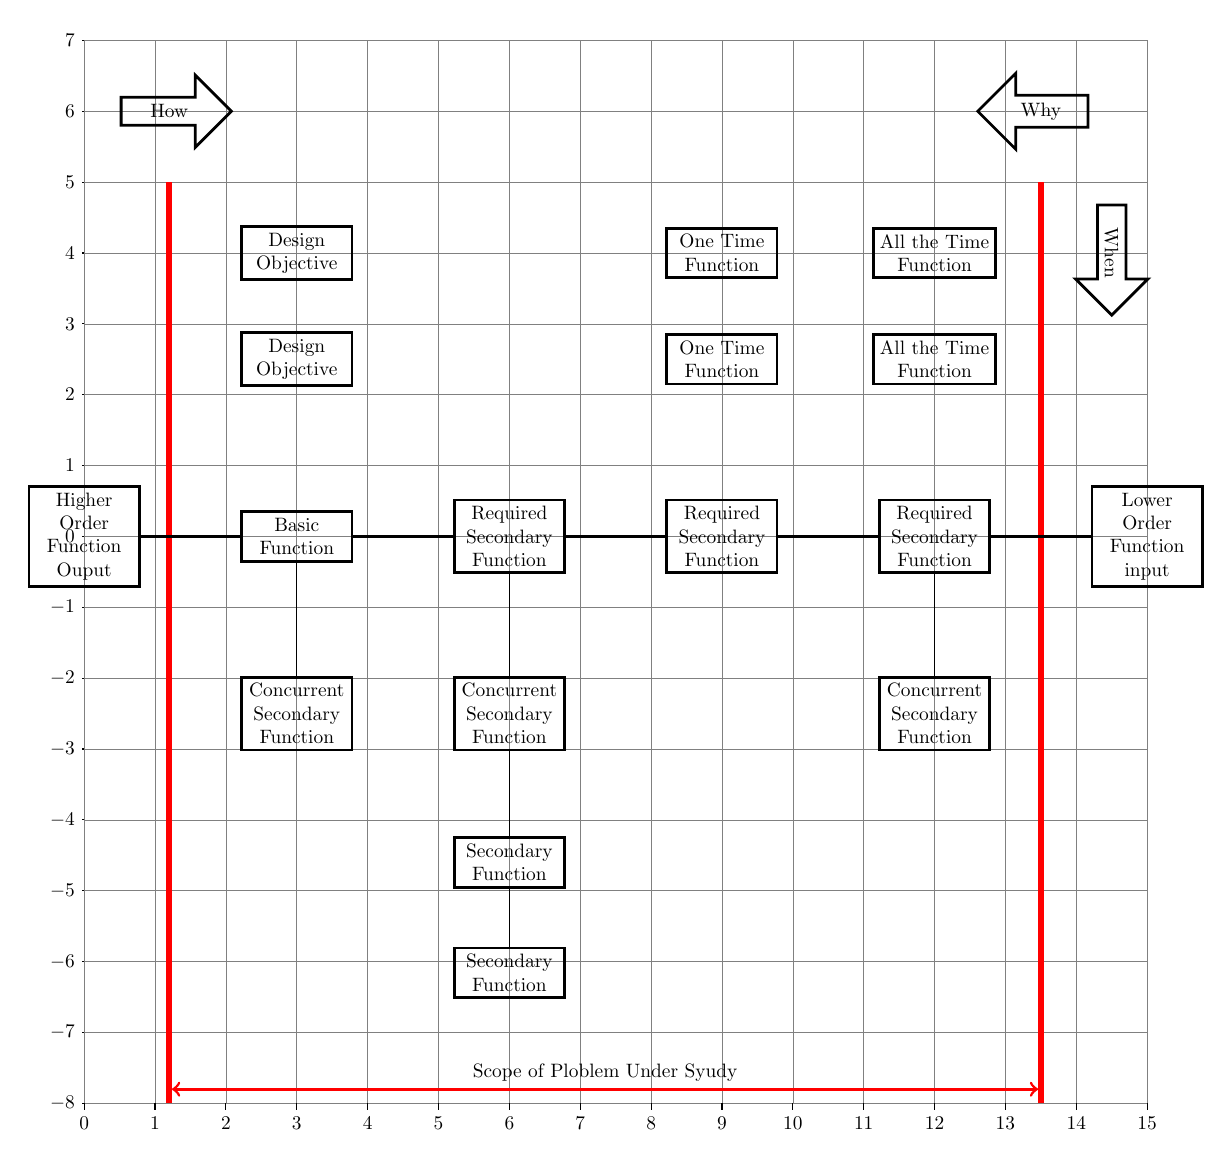
\begin{tikzpicture}[	scale=0.9, 
							every node/.style={scale=0.7},
							node distance=2.0cm,
						]
			% ---------------------------------------  draw grid
			\draw[help lines] (0,-8) grid (15,7);
			% x
			\foreach \x in {0,1,...,15}
			\draw (\x cm,-8cm) -- (\x cm, -8.1cm) node[anchor=north] {$\x$};
			% y
			\foreach \y in {-8,-7,...,7}
			\draw (0, \y cm) -- (-1pt, \y cm) node[anchor=east] {$\y$};


			\tikzstyle{block} = 	[draw, line width=1pt,
								shape=rectangle,
								align=center,
								minimum width=2.0cm,
								minimum height=1.5em,
%								text width=2cm,
								shape=rectangle,
								rounded corners=0.0em];

			\tikzstyle{rblock}=[	draw, 
								align=center,
								minimum width=3.0em,
								minimum height=1.5em,
								text width=5.0em,
								shape=rectangle,
								rounded corners=0.5em];

			% -----------------------
			\draw [red, line width=2pt] ( 1.2,5) -- (1.2,-8);
			\draw [red, line width=2pt] (13.5,5) -- (13.5,-8);
			\draw [red, line width=1pt, |<->|] (1.2,-7.8) -- (13.5,-7.8) 
				node [midway, above, black]{Scope of Ploblem Under Syudy };

			% -----------------------
			\node [	single arrow, draw,line width=1pt,
					rotate=0,
					minimum height=2cm,
					single arrow head extend=0.4cm ,
					single arrow head indent=0.0cm 
					] 
					at(1.2,6) (C00) {How};
			\node [	single arrow, draw,line width=1pt,
					shape border rotate=180,
					minimum height=2cm,
					single arrow head extend=0.4cm ,
					single arrow head indent=0.0cm 
					] 
					at(13.5,6) (C00) {Why};
			\node [	single arrow, draw,line width=1pt,
					rotate=-90,
					minimum height=2cm,
					single arrow head extend=0.4cm ,
					single arrow head indent=0.0cm 
					] 
					at(14.5,4) (C00) {When};



			\node [block] 				(B00) {Higher\\ Order\\Function \\Ouput};
			\node [block] at(3,0) 			(B11) {Basic \\Function};
			\node [block] at(6,0)		 	(B21) {Required\\Secondary\\Function};
			\node [block] at(9,0)		 	(B31) {Required\\Secondary\\Function};
			\node [block] at(12,0) 		(B41) {Required\\Secondary\\Function};
			\node [block] at(15,0) 	 	(B51) {Lower\\Order\\Function\\input};

			\draw[-,line width=1pt] (B00) -- (B11);
			\draw[-,line width=1pt] (B11) -- (B21);
			\draw[-,line width=1pt] (B21) -- (B31);
			\draw[-,line width=1pt] (B31) -- (B41);
			\draw[-,line width=1pt] (B41) -- (B51);


			\node [block] at(3,-2.5)	 	(B12) {Concurrent\\Secondary\\Function};
			\draw[-,line width=0pt] (B11) -- (B12);

			\node [block] at(6,-2.5)	 	(B22) {Concurrent\\Secondary\\Function};
			\node [block, below of=B22,yshift=-2em] 	(B23) {Secondary\\Function};
			\node [block, below of=B23,yshift=0em] 	(B24) {Secondary\\Function};
			\draw[-,line width=0pt] (B21) -- (B22);
			\draw[-,line width=0pt] (B22) -- (B23);
			\draw[-,line width=0pt] (B23) -- (B24);


			\node [block] at(12,-2.5)	 	(B42) {Concurrent\\Secondary\\Function};
			\draw[-,line width=0pt] (B41) -- (B42);


			% Design Objective
			\node [block] at(3.0, 4) 		(A01) {Design\\Objective};
			\node [block] at(3.0, 2.5)		(A02) {Design\\Objective};

			% One Time Function
			\node [block] at(9.0, 4) 		(A01) {One Time\\Function};
			\node [block] at(9.0, 2.5)		(A02) {One Time\\Function};

			% All the Time Function
			\node [block] at(12.0, 4) 		(A01) {All the Time\\Function};
			\node [block] at(12.0, 2.5)		(A02) {All the Time\\Function};
			
			\draw[-,line width=1pt] (B00) -- (B11);

		\end{tikzpicture}






% ===========================================================	part		=============
		\addtocontents{toc}{\protect\newpage}
		\part{타이틀 페이지}



% 	================================================= chapter 	====================
%   		타이틀 페이지
%	-------------------------------------------------------------------------------
	%	---------------------------------------------------------------------------
		\newpage
		\section{타이틀 페이지 만들기}


		\begin{enumerate}[leftmargin=2.0em]
		\item	1 Standard Title Pages
		\item	2 Custom Title Pages
				\begin{enumerate}
				\item	2.1 Create the title
				\item	2.2 A practical example
				\item	2.3 Integrating the title page
				\end{enumerate}
		\item	3 Packages for custom titles
		\item	4 Notes and References
		\end{enumerate}





	%	---------------------------------------------------------------------------
		\newpage
		\section{Standard Title Pages}




	%	---------------------------------------------------------------------------
		\newpage
		\section{간단한 타이틀 페이지}




		\begin{titlepage}
		    \begin{center}
				\vspace*{1cm}
				\rule{1.0\textwidth}{0.5mm}
				\Huge
				\textbf{보고서 제목}\\
				\rule{1.0\textwidth}{0.5mm}
				\vspace{0.5cm}
				\Large
				보고서 부제목\\
				\vspace{1.5cm}
				\textbf{Author Name}\\
				\vfill
		        
		        A thesis presented for the degree of Doctor of Philosophy
		        
		        \vspace{0.8cm}
		        
		%        \includegraphics[width=0.4\textwidth]{university}
		        
				\Large
				Department Name\\
				University Name\\
				Country\\
				Date
				\vspace{2.0cm}
		    \end{center}
		\end{titlepage}





	%	---------------------------------------------------------------------------
		\newpage
		\section{간단한 타이틀 페이지}



		\begin{titlepage}

			\newgeometry{left=7.5cm} %defines the geometry for the titlepage

		% -----------------------------------------------	
		% 페이지 칼라 제어
		% -----------------------------------------------	

%			\usepackage{xcolor}
%			\usepackage{afterpage}
			\pagecolor{black} \afterpage{\nopagecolor{}}
			\color{white}


		    \begin{center}
				\vspace*{1cm}
				\rule{1.0\textwidth}{0.5mm}
				\Huge
				\textbf{보고서 제목}\\
				\rule{1.0\textwidth}{0.5mm}
				\vspace{0.5cm}
				\Large
				보고서 부제목\\
				\vspace{1.5cm}
				\textbf{Author Name}\\
				\vfill
		        
		        A thesis presented for the degree of Doctor of Philosophy
		        
		        \vspace{0.8cm}
		        
		        
				\Large
				Department Name\\
				University Name\\
				Country\\
				Date
				\vspace{2.0cm}
		    \end{center}
		\end{titlepage}






% 	================================================= chapter 	====================
%   		타이틀 페이지
%	-------------------------------------------------------------------------------
		\newpage
		\chapter{타이틀 페이지 : use fancycyhdr }





				%	----------------------------------------------------
				%	문서 표지 페이지
				%	----------------------------------------------------
					\begin{titlepage}
					\begin{center}
					\vspace*{1cm}  %	----------------- 윗부분 여백지정
					\rule{1.0\textwidth} {0.1mm}
					\Huge  \textbf{\hspace*{1cm} \hfill 보와 골조 \hfill \hspace{2cm}} 
					\par
					\rule{1.0\textwidth} {0.1mm}
					% ----------------------------------
					\vspace{0.5cm}
					\Large 전단력과 휨모멘트
					\par
					% ----------------------------------
					\vfill
					2015년 7월
					\vfill
					% ----------------------------------
					\textbf{김 대희}
					\par
					\vspace{1.5cm}
					\Large 서영엔지니어링 양산감리단
					\par
					\vspace{2.0cm}  %	----------------- 아래부분 여백 정의
					\end{center}
					\end{titlepage}
				%	----------------------------------------------------





	% ------------------------------------------------------------------------------
	%	Maketitle
	% ------------------------------------------------------------------------------
		\begin{titlepage}

		\singlespace
		\pagestyle{empty}
		\newcommand{\HRule}{\rule{\textwidth}{0.5mm}}

		\begin{center}
		\null
		\vspace{2cm}
		\textsc{\LARGE Value Engineering}\\[1.0cm]
		\HRule\\[-0.4cm]
		\HRule \\[0.4cm]
			{ \huge \bfseries 설계의 경제성 등 검토 \\[0.4cm] }
		\HRule\\[-0.4cm]
		\HRule \\[1.5cm]
		
		% Author and supervisor
		\noindent
		\begin{minipage}{1\textwidth}
			\begin{flushright} \large \emph{Author:}  김대희	\end{flushright}
		\end{minipage}%
		\vfill
		% Bottom of the page
		{\large \today}
		
		\end{center}
		\cleardoublepage
		\end{titlepage}																						



	% ------------------------------------------------------------------------------
	%	Maketitle
	% ------------------------------------------------------------------------------
			\begin{titlepage}
			\thispagestyle{empty}				% Remove page numbering on this page
			\definecolor{grey}{rgb}{0.9,0.9,0.9} 
			\colorbox	{grey}
						{ \parbox[t]{1.0\linewidth}
						{
						\vspace*{1.2cm} 
						\fontsize{20}{20} \rmfamily \hfill \today 		\\ [0.8cm] \null
						\fontsize{40}{20} \rmfamily \hfill Value Engineering \\ [0.8cm] \null
						\fontsize{20}{50} \rmfamily \hfill ver101
						\vspace*{0.8cm} 
						} }
			\vfill
			% Print the author data as defined above
			\hfill Kim Dae Hee\\ \null
			\hfill (주)서영엔지니어링\\ \null
			\hfill 건설관리팀\\ \null
			\hfill \url{h01038395609@gmail.com} \\ \null
			\hfill \rule{0.4\linewidth}{1pt}
			\end{titlepage}
			\clearpage

	% ------------------------------------------------------------------------------
	%	Maketitle
	% ------------------------------------------------------------------------------

				\newpage   
				\thispagestyle{empty}
				\begin{center}
				\null
				\vspace{6em} % White space at the top of the page
		
				\rule{\textwidth}{1.6pt}\\[-1.9em]%\vspace{0.1pt} % Thick horizontal line
				\rule{\textwidth}{0.4pt}\\[2em]
		
				{\Huge 중점 품질 관리 대상 }\\[1.0em]
		
				\rule{\textwidth}{0.4pt}\\[-1.7em]
				\rule{\textwidth}{1.6pt}
				\end{center}



	% ------------------------------------------------------------------------------
	%	환경 정의 : 박스 치고 안의 글자 파란색
	% ------------------------------------------------------------------------------

		\newpage
	% --------------------------------- 

			\newenvironment{typing_code}
			{ 	\setlength{\fboxsep}{12pt}
				\begin{boxedminipage}[c]{1.0\linewidth}
				\color{blue}
			}
			{ 	\end{boxedminipage} 
				\color{black}
			}


			\begin{typing_code}
			code 입력
			\end{typing_code}
			

























% ------------------------------------------------------------------------------
% End document
% ------------------------------------------------------------------------------
\end{document}


